%!TEX program = pdflatex
\documentclass{elegantpaper}
\usepackage{listings}% http://ctan.org/pkg/listings
\lstset{
	basicstyle=\ttfamily,
	mathescape
}

\title{Project 5: Rolling your own CDN}
\author{{Yunfan Tian} 
		 \\[0.5ex] %
		College of Engineering}
\date{\small\itshape  \today}

\begin{document}
\maketitle

\begin{abstract}
	This project illustrates the design thought process of rolling out my own CDN. It contains the explanation of various components of CDN, HTTP server design especially the cache replacement strategy, and the algorithm to select replica server for each client request. If you have any questions or suggestions, please contact me at: \email{tian.yun@husky.neu.edu}.
\end{abstract}

\section{Introduction}

The idea of a CDN is to distributed a collection of \textit{server surrogates} that cache pages normally maintained in some set of \textit{back-end servers}. Thus, it is possible to spread the load of web requests across many servers. Direct clients to replica server will improve the performance of HTTP requests. Clearly, it's expensive for a single site to maintain a lot of replica servers, but commercial CDN provide this service for many sites, thereby amortizing the cost across many customers\cite{Peterson}.

\section{Key Components}
The main components of CDN is a large set of distributed servers, they usually  located inside of other ISPs or IXPs. High-speed network connects those servers, and Glue binds those clients who wants fast Web performance to "nearby" replica servers. Moreover, a system determines how to map clients to "good" replica servers is also the key component.
\begin{figure}[!ht]
	\centering
	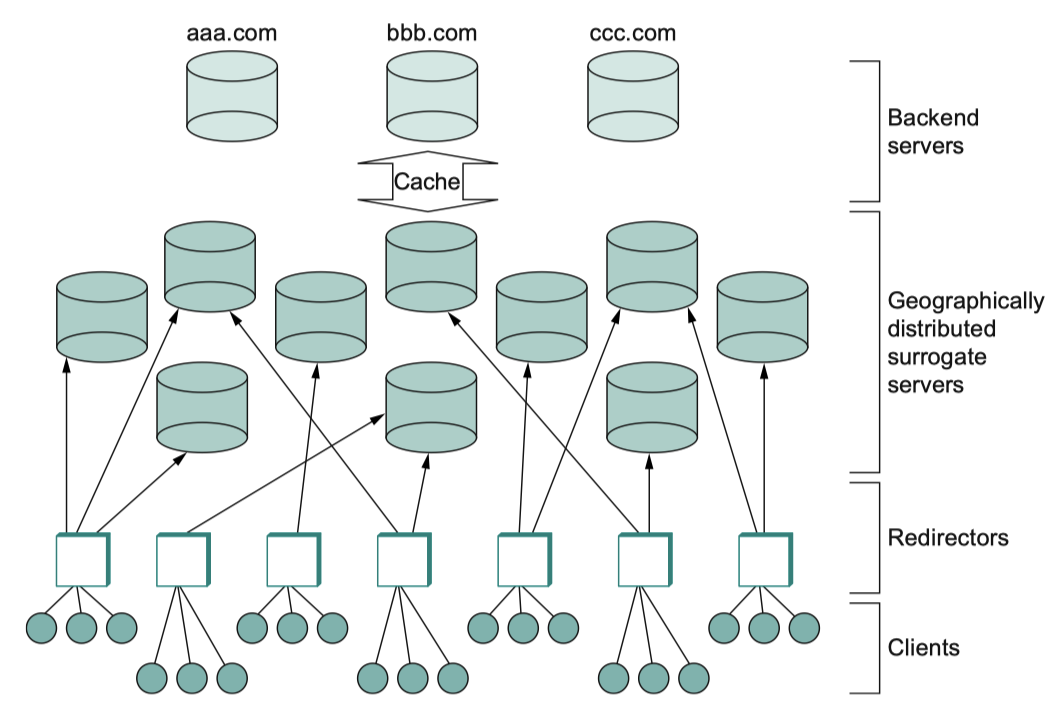
\includegraphics[width=0.6\textwidth]{CDNs.png}
	\caption{Components in a Content Distribution Network (CDN)\label{fig:cdn}}
\end{figure}
\subsection{Distributed Servers}
We can view replica servers as caches. They ask the backend server for a page if they don't have the requested page. In practice,  the backend servers proactively replica their data across the surrogates rather than wait for surrogates to request it. It's only the case for static pages, customers have to go to the backend servers for dynamic or customized content (e.g., banking content)
\subsection{System Determines Mappings}
Having a large set of geographically distributed servers does not fully solve the problem. CDNs also need to provides a set of redirectors that forward client requests to the most appropriate server. The primary objective of redirectors is to select the server with best \textit{response time} for each request, the second objective  is to process as many requests as possible per second under hardware restriction. 

CDNs use several factors to decide how to map client requests. A redirector may select a server based on \textit{network proximity} to minimize response time; or \textit{balance} the load across servers to improve overall system throughput. In both cases, the distribution mechanism should take \textit{locality} into consideration. 

Redirection could be implemented by existing, scalable DNS infrastructure, it will help to keep the URLs stay essentially the same. For example, when a client asks to resolve the name cs5700cdn.example.com, the DNS server could return the IP address of a server hosting cs5700cdn Web pages that having lightest load. DNS may select servers in a round-robin fashion or use some hashing algorithm.

\section{HTTP server design}
The size of the content at the origin server is much larger than the size of cache on a replica server. if a replica server don't have the content which clients requested, clients have to ask the original server for it. So, CDN must implement a cache replacement strategy to keep content popular.

\subsection{Cache Replacement Strategies}
The cache replacement policies refer to deciding which objects will evict from the cache to accommodate new objects\cite{CaTech}. There are several well-known cache replacement algorithms: 
\begin{enumerate}
	\item \textbf{First-In, First-Out (FIFO)}. All objects are stored in a queue, when the buffer is full, the first object in the head of the queue will be replaced, regardless of its popularity and demand.
	
	\item \textbf{Least Recently Used (LRU) Algorithm}. Replacing the object in cache that is accessed least recently.
	
	\item \textbf{Least Frequently Used (LFU) Algorithm}. If an object is not requested for some time, then it will be replaced despite the fact it may be requested frequently over time\cite{Cache}.
	
	\item \textbf{Least Frequent Recently Used (LFRU)}. The cache is divided into privileged and unprivileged partitions. The privileged partitions use the LRU replacement policy while the unprivileged partition employs an approximated LFU\cite{7857720}. 
	
	\item \textbf{SIZE Algorithm}. Object size is treated as the promary factor when caching the object. When buffer is full, it removes web object with the biggest size\cite{8344541}.
	
	\item  \textbf{Balady's Algorithm}. This algorithm would be to always discard the information what will not be needed in the future. It's generally impractical because it's hard to predict which object will be needed in the future.
\end{enumerate}

\subsection{My Choice: LFRU}
LFRU cache replacement scheme combines the benefits of LFU and LRU schemes. The cache has privileged and unprivileged partitions. The privileged partition can be defined as a protected partition. If content is highly popular, it is pushed into the privileged partition. LFRU use LFU to evicts object from unprivileged partition, then insert new content to privileged partition, and use LRU to evict object in privileged partition.

We calculated the priority of content based on the arrival rate and size of the content\cite{7857720}. The basic idea is to filter out the locally popular contents with LFU scheme and push the popular contents to privileged partition.

In our project, the cache is changed rapidly and content size in CDNs is much smaller than original server. LFRU could help keep real high popularity content in privileged partition and replace least popular content rapidly.

\section{Determine Replica Servers}
CDNs rely on the DNS for replica server selection\cite{CDN1}. \textit{Network proximity} and \textit{load balance} are two main properties used for choosing replica servers, one is to minimize response time, the other one is to improve overall system throughput. If the distribution mechanism takes \textit{locality} into consideration, both response time and throughput will improve. That means select a server already have requested page in cache.

The mapping system should also take other properties into account, such as server side usage, latency period, the average transfer rate, packet loss rate and geographic proximity\cite{CDN2}. The weighting of factors depends on the data that's being requested. In this project, we use time-to-completion (TTC) for downloading a Web page to evaluate performance, so the average transfer rate and latency is much more important.

\subsection{Hashing Schemes}
We uses some form of hashing to deterministically map URLs into a small range of values\cite{Wang:2002:ERR:844128.844160}. The choice of which hashing style to use is one component of the design space, and is somewhat flexible.
\begin{enumerate}
	\item \textbf{Modulo Hashing}, the URL is hashed to a number of servers.
	\item \textbf{Consistent Hashing}, the URL is hashed to a number in a large, circular space, as are the names of the servers. The URL is assigned to server that lies closest on the circle to its hash value.
	\item \textbf{Highest Random Weight}, This approach consists of generating a list of hash values by hashing the URL and each server's name by random weights and sorts result. It's the basis for CARP.
\end{enumerate}
Since we choose CARP in the next section, I will give more details in HRW. The basic idea is to give each site $S_j$ a score for each object $O_i$. For object $O_i$, the site $S_j$ is defined to have weight $w_{i,j}=h(O_i,S_j)$. HRW assigns $O_i$ to the site $S_m$ whose weight $w_{i,m}$ is the largest. Each client can independently compute the weights $w_{i,1}, w_{i,2},...,w_{i,n}$ and pick the largest value. If a site is added or removed, only the objects mapping to S need to re-hash\cite{HRW}.

\subsection{My Choice: CARP}
There are several request redirection strategies, such as Random, Static Server Set, Load-Aware Static Server Set, Dynamic Server Set and so on. I choose Cache Array Routing Protocol (CARP) in my design for:
\begin{itemize}[noitemsep]
	\item This strategy take server load into account. We use the count of how many requests a redirector forward to a server to estimate the server's current load.
	\item CART could select the highest weight server below threshold. This help to fully utilize each server.
	\item If one server fails its load is distributed evenly among the other machines.
\end{itemize}
\textbf{Pseudo-code for CARP:}
\begin{Verbatim}[tabsize=4,frame=single,baselinestretch=1]
SelectServer(URL, S)
	for = each server s_i in server set S
		weight_i = hash(URL, address(s_i))
	sort weight
	for each server s_j in decreasing order or weight_j
		if = Load(s_j) < threshold then
			return s_j
	return server with highest weight
\end{Verbatim}
As load increases, CARP spread requests across several servers. Servers having popular pages may find more servers sharing their load. In this process, if some pages become extremely popular, it's possible that all of the servers in the system could serve them.

\subsection{Network Proximity}
It is also possible to introduce network proximity into the above algorithm. In my project, average transfer rate and latency are main factors, choose nearby/lightest loaded servers could significantly improve the performance. There are two ways to introduce network proximity.

First, monitor how long a server response to requests and using this as the "server load" parameter in the preceding algorithm. This strategy tends to choose nearby/lightly loaded server.

Second, consider nearby set of servers at earlier stage in above algorithm. One approach is to select available servers in same ISP. Another more sophisticated approach is look at the AS map produced by BGP and select only those servers within some number of hops from client.

In our project, we  use time to complete (TTC) download to evaluate performance. Using response time to factor network proximity would be better help to improve the average transfer rate.



\bibliographystyle{acm}
\bibliography{wp_ref}
\end{document}
